%% =====================================================================
%% What Changed in the Room, a guide to the project
%% Ramdas Narayan Chaugale
%%
%% Build:  pdflatex main.tex   (run twice for the contents)
%% Each part is its own file under parts/, so one can be edited alone.
%% =====================================================================

\documentclass[11pt,a4paper]{report}

\usepackage[T1]{fontenc}
\usepackage[utf8]{inputenc}
\usepackage[english]{babel}
\usepackage{lmodern}

\usepackage[top=22mm,bottom=22mm,left=25mm,right=25mm]{geometry}
\usepackage{graphicx}
\usepackage{booktabs}
\usepackage{amsmath,amssymb}
\usepackage{xcolor}
\usepackage{enumitem}
\usepackage{caption}
\usepackage{fancyhdr}
\usepackage{titlesec}
\usepackage{listings}
\usepackage[hidelinks]{hyperref}
\usepackage{tikz}
\usepackage{tcolorbox}
\usetikzlibrary{arrows.meta, positioning, fit, backgrounds, calc}

\graphicspath{{../figures/}{../../examples/inputs/}}
\setlist{nosep,leftmargin=*,topsep=5pt,partopsep=0pt}
\captionsetup{font=small,labelfont=bf}
\emergencystretch=3em

\definecolor{boxblue}{RGB}{224,236,250}
\definecolor{boxgrey}{RGB}{242,242,242}
\definecolor{boxgreen}{RGB}{226,243,228}
\definecolor{boxamber}{RGB}{253,243,220}
\definecolor{linkblue}{RGB}{30,80,150}
\definecolor{codebg}{RGB}{247,247,244}
\definecolor{codekey}{RGB}{20,90,150}
\definecolor{codecom}{RGB}{110,115,120}

\lstset{
  basicstyle=\ttfamily\small,
  backgroundcolor=\color{codebg},
  keywordstyle=\color{codekey}\bfseries,
  commentstyle=\color{codecom}\itshape,
  stringstyle=\color{codekey},
  showstringspaces=false,
  breaklines=true,
  frame=leftline,
  framerule=1.2pt,
  rulecolor=\color{codekey!35},
  xleftmargin=10pt,
  framexleftmargin=8pt,
  aboveskip=9pt,
  belowskip=9pt,
  language=Python,
}

% where this idea shows up in the project
\newtcolorbox{project}[1][]{
  colback=boxgreen, colframe=boxgreen!60!black, boxrule=0.4pt,
  left=6pt, right=6pt, top=5pt, bottom=5pt,
  title={\bfseries In this project}, fonttitle=\small, #1}

% a plain definition
\newtcolorbox{plainbox}[1][]{
  colback=boxblue, colframe=boxblue!60!black, boxrule=0.4pt,
  left=6pt, right=6pt, top=5pt, bottom=5pt, #1}

% a warning or a common misunderstanding
\newtcolorbox{watch}[1][]{
  colback=boxamber, colframe=boxamber!60!black, boxrule=0.4pt,
  left=6pt, right=6pt, top=5pt, bottom=5pt,
  title={\bfseries Watch out}, fonttitle=\small, #1}

\pagestyle{fancy}
\fancyhf{}
\fancyhead[L]{\small\nouppercase{\leftmark}}
\fancyhead[R]{\small\thepage}
\renewcommand{\headrulewidth}{0.3pt}

\titleformat{\chapter}[display]
  {\normalfont\huge\bfseries}{\chaptertitlename\ \thechapter}{16pt}{\Huge}
\titlespacing*{\chapter}{0pt}{-20pt}{24pt}

\begin{document}

\begin{titlepage}
\centering
\vspace*{2.6cm}
{\Huge\bfseries What Changed in the Room?\par}
\vspace{1.2cm}
{\Large A guide to the project, assuming nothing\par}
\vspace{2.2cm}
{\large Ramdas Narayan Chaugale\par}
\vspace{6pt}
{\large MSc Artificial Intelligence\par}
{\large Queen's University Belfast\par}
\vspace{1.6cm}
\begin{minipage}{0.84\textwidth}
\small
This project takes two phone videos of the same room, filmed at different times, and works out what
moved, what appeared and what is gone, in three dimensions.

\vspace{6pt}
These notes are written so that someone with no technical background can follow what it does and
why. Chapter 1 stands on its own. Each chapter after that assumes a little more, and every tool is
explained in plain words before it is used.

\vspace{8pt}
\textbf{1} what it is, with no jargon at all.
\textbf{2} why it exists, and why a robot would want it.
\textbf{3} every tool, what it does here, and why it was chosen over the alternatives.
\textbf{4} what actually happens, step by step.
\textbf{5} the decisions that mattered.
\textbf{6} the fake room used to check the answers.
\textbf{7} a glossary.
\textbf{8} the questions worth being ready for, including what went wrong.

\vspace{8pt}
The hard part of this problem is not spotting that something is different. It is being sure that an
empty space means the object left, rather than that nobody looked there.
\end{minipage}
\vfill
{\small \today}
\end{titlepage}

\tableofcontents

\chapter{What this is, in plain words}

Imagine you film a short video walking around your living room on Monday. On Friday somebody moves
the armchair, takes away a cardboard box, and leaves a rucksack by the door. You film the room
again.

This project takes those two videos and tells you:

\begin{itemize}
  \item the armchair moved, and roughly how far
  \item the box is gone
  \item a rucksack appeared
  \item the table did not move
\end{itemize}

It also shows this as a three dimensional model you can spin round in a web browser, with the
things that changed picked out in colour. Nobody has to tell it what to look for. It works out the
shape of the room from the videos themselves.

\section{Why that is harder than it sounds}

If you simply compared the two videos frame by frame, almost everything would look different. You
stood in a different spot. You held the phone at a different angle. You walked a slightly different
route. The light changed.

The genuinely hard part is not spotting that something is different. It is being certain that an
empty space means \textbf{the object was taken away} rather than \textbf{I just did not point the
camera there the second time}.

\begin{watch}
A person does this without thinking. A computer has to be told the difference, and most systems get
it wrong: they report everything the camera missed as a change. On real footage, where nobody walks
the identical route twice, that is most of the room.
\end{watch}

That problem is what the whole project is built around, and Chapter~4 explains the two ideas that
solve it.

\section{What goes in}

Two ordinary phone videos of the same room, twenty to sixty seconds each, walked along a similar
route. Nothing else. No special camera, no depth sensor, no markers placed in the room, no
measurements taken by hand.

\begin{figure}[h]
\centering

\includegraphics[width=\textwidth]{before_after.jpg}
\caption{Three matching moments from the two recordings used to test the system, before on the left
and after on the right. This is a drawn test room rather than a real one, for reasons explained in
Chapter~6.}
\end{figure}

\section{What comes out}

Three things.

\begin{itemize}
  \item \textbf{An interactive 3D scene} in a web browser. The unchanged room is grey, removals are
        red, additions are green, moves are amber. You can drag to rotate it.
  \item \textbf{A written summary} in ordinary English, for example: ``A chair moved. It was in the
        centre on the left side and is now towards the back on the right side, about 2.4 m away.''
  \item \textbf{A data file} listing every change with its position, size, name and the evidence
        behind the naming, for anything that needs to read the result automatically.
\end{itemize}

\chapter{Why it exists}

It was built as a technical challenge for a job application to Humanoid, a London company building
humanoid robots. Their brief was to compare two phone recordings of a room and identify meaningful
changes in three dimensions, while distinguishing genuine change from differences in camera
viewpoint, occlusion and incomplete observation.

That last clause is the whole exercise. Anyone can write something that notices two pictures are
not identical. The brief asks for something that knows when it is entitled to say so.

\section{Why a robot would want this}

A robot working in a warehouse, a hospital or a home builds a map of its surroundings. The world
then moves. Pallets get shifted. Doors close. Boxes appear in corridors. Furniture is rearranged
around it. The robot has to notice, without being re-shown the whole building every morning.

\begin{plainbox}
\textbf{The consequence of being wrong is not symmetrical.}

If the robot wrongly believes a chair is still there, it goes around a chair that is not there. It
wastes a few seconds.

If the robot wrongly believes a corridor is clear, because it never actually looked, it drives into
something.
\end{plainbox}

So a system like this should prefer saying \emph{I do not know} over guessing. That single
principle runs through every design decision in the project, and it is why the system is
deliberately built to under-report rather than over-report.

\section{Why it is not solved already}

Depth cameras and laser scanners make this much easier, and plenty of robots carry them. This
project deliberately uses nothing but an ordinary phone camera, because the brief said phone
recordings.

That removes the one thing that would make the problem simple, which is a direct measurement of
distance. Everything about distance here has to be inferred from how the view changes as the camera
moves, and from a model that has learned what near and far look like. Chapter~3 covers both.

\chapter{Every tool, and why}

Each tool gets a plain explanation, then what it does in this project, then why it was chosen over
the alternatives.

\section{COLMAP, used through pycolmap}

\begin{plainbox}
\textbf{What it is.} Software that works out the three dimensional shape of a scene from ordinary
two dimensional photographs, and where the camera was standing for each one. The technique is
called \emph{structure from motion}. It is the same idea your eyes use: two slightly different
views of the same thing let you judge depth.
\end{plainbox}

\begin{project}
It takes every frame from both videos and returns two things. First, the position and angle of the
camera for each frame. Second, a sparse cloud of three dimensional points marking corners and edges
it managed to recognise in several frames at once.
\end{project}

\textbf{Why this one.} It is the standard tool for the job and it is free. The Python package
\texttt{pycolmap} installs with pip, so there is no separate program to set up, which matters when
somebody else has to run your work. A robotics team will recognise it immediately.

\section{Depth Anything V2}

\begin{plainbox}
\textbf{What it is.} A neural network that looks at a single photograph and estimates how far away
every pixel is. It was trained on an enormous number of images, so it has learned the cues that
make things look near or far: perspective, relative size, and how objects overlap each other.
\end{plainbox}

\begin{project}
COLMAP returns a few hundred accurate points per frame, which is nowhere near enough to say whether
a chair is standing in a corner. This fills in a depth estimate for every single pixel.
\end{project}

\textbf{Why this one.} It runs on a laptop with no dedicated graphics card. The textbook
alternative, dense multi-view stereo, is more accurate but effectively requires a powerful GPU,
which would have made the project impossible to run or review on an ordinary machine.

\begin{watch}
Its output has no sense of scale. It knows the sofa is nearer than the wall; it does not know the
sofa is two metres away. Section~4.3 explains how that is fixed, and it is one of the more
interesting parts of the project.
\end{watch}

\section{CLIP}

\begin{plainbox}
\textbf{What it is.} A model trained on hundreds of millions of image and caption pairs. Give it a
picture and a list of candidate descriptions, and it scores how well each description fits. It was
never trained on a fixed list of objects, so the list can be changed without retraining anything.
\end{plainbox}

\begin{project}
Once the geometry has found a lump of space that changed, CLIP is shown a cropped photograph of
that space and picks the best match from a list of household objects, so the final report says
``a chair'' instead of ``cluster 3''.
\end{project}

\textbf{Why this one.} The geometry has already decided \emph{where} the object is, so a full
object detector is not needed, only a name. CLIP is small, runs on a laptop, and needs no training
data.

\section{DBSCAN, from scikit-learn}

\begin{plainbox}
\textbf{What it is.} An algorithm that finds groups in scattered data. Unlike most clustering
methods, you do not tell it how many groups to expect. It finds however many there are, and labels
loose scattered points as noise rather than forcing them into a group.
\end{plainbox}

\begin{project}
After the comparison there are thousands of individual cells of space marked as changed. DBSCAN
groups touching cells into objects, turning ``four thousand changed cells'' into ``a chair sized
lump here and a box sized lump over there''.
\end{project}

\textbf{Why this one.} Not knowing the number of objects in advance is the entire point, which
rules out anything that needs that number up front. Its willingness to discard scattered points as
noise is exactly what is wanted, because measurement error produces scattered points.

\section{OpenCV}

\begin{plainbox}
\textbf{What it is.} The standard library for working with images and video in code.
\end{plainbox}

\begin{project}
Reads the videos, pulls out frames, resizes them, and measures how blurry each one is so the bad
ones can be discarded. It also draws the synthetic test room described in Chapter~6.
\end{project}

\section{Plotly}

\begin{plainbox}
\textbf{What it is.} A charting library that produces interactive graphics which open in a web
browser.
\end{plainbox}

\begin{project}
Produces \texttt{scene.html}, the rotatable three dimensional model of the result.
\end{project}

\textbf{Why this one.} The output is a single file that opens in any browser. The usual
alternative for 3D work, Open3D, opens a desktop window instead, which is no use to somebody
reviewing the work from a link.

\section{Matplotlib}

\begin{plainbox}
\textbf{What it is.} The standard Python library for charts.
\end{plainbox}

\begin{project}
Draws the figures used in this document and in the project's README. They are generated from the
real output of a real run rather than drawn by hand, so they cannot quietly drift away from what
the code actually produces.
\end{project}

\section{NumPy}

\begin{plainbox}
\textbf{What it is.} The library that lets Python do arithmetic on millions of numbers quickly.
\end{plainbox}

\begin{project}
Everything numerical. The free space calculation described in Section~4.4 handles tens of millions
of points. In ordinary Python that would take hours. In NumPy it takes seconds.
\end{project}

\chapter{What actually happens, step by step}

\section{Turn the videos into pictures}

Sample a couple of frames per second, shrink them, and throw away the blurry ones. Blur is measured
by how sharp the edges are in the picture.

A blurry frame is worse than no frame at all, because the next stage works by recognising the same
corner in several different pictures, and blur destroys corners.

\section{Work out the shape of the room, from both videos at once}

\begin{watch}
This is the single most important decision in the project. If only one thing is remembered from
these notes, it should be this section.
\end{watch}

The obvious approach is to build a three dimensional model from video A, build a second one from
video B, and then line the two up.

That approach asks the hardest question first. Lining up two models works by finding the position
where they best agree, and it is least reliable exactly when part of the scene has genuinely moved.
The things that changed drag the alignment off, and once the alignment is wrong, everything looks
changed.

So instead, every frame from \textbf{both} videos goes into \textbf{one} reconstruction. The walls,
the floor and the furniture that stayed put appear in both recordings, so the software matches them
across the two videos by itself, and everything emerges in a single shared coordinate system. There
is no lining up step to get wrong.

\begin{plainbox}
Put simply: \textbf{the parts of the room that did not change are what tie the two visits
together}. The stable scene is the evidence. The changes are the thing being measured. Doing it the
other way round uses the unknown to establish the evidence.
\end{plainbox}

The code refuses to continue if both videos did not end up in the same model. A model containing
only video A would report the whole of video B as new, and that would look like a result rather
than a failure.

\section{Fill in the depth, and fix the scale}

The points from the previous step are accurate but sparse. Depth Anything fills in every pixel, but
its output has no scale.

The fix uses one against the other. Both describe the same frame, so finding the stretch and shift
that makes the estimated depths line up with the accurate sparse points converts the whole dense
estimate into the same units as the reconstruction. One small calculation per frame, and the dense
depth inherits whatever scale the reconstruction has.

Frames with too few sparse points to do this reliably are skipped rather than guessed at.

\begin{watch}
A wrongly scaled depth map does not produce a slightly wrong answer. It produces a confident answer
in completely the wrong part of the room, which is far more damaging than no answer.
\end{watch}

There is one further wrinkle. Reconstruction from photographs alone can never recover true
real-world size, because a doll's house photographed close up looks identical to a real house
photographed from further away. So the whole scene is rescaled once, so that typical distances come
out room sized. This is not true measurement, but it makes every setting in the configuration file
mean roughly what it appears to mean.

\section{Record what each visit knows, including what was empty}

Space is divided into a grid of cells, each five centimetres across. For each visit, every cell is
marked as one of three things.

\begin{center}
\begin{tabular}{@{}ll@{}}
\toprule
\textbf{Label} & \textbf{Meaning} \\
\midrule
occupied & something was measured here \\
free & a camera ray passed through here on its way to hitting something \\
 & further away, so this space was looked at and was empty \\
unknown & neither, so nothing can be said about it \\
\bottomrule
\end{tabular}
\end{center}

\textbf{Free is the state that makes this work.} Finding it means tracing the straight line from
the camera out to each thing it saw, and marking everything along the way as confirmed empty. It is
the most expensive part of the whole program and it is the reason the results can be trusted.

The tracing stops slightly short of the surface. Without that margin, the front face of every
object would erase itself and solid things would dissolve.

\section{Compare}

Two rules, and the whole argument of the project sits in them.

\begin{lstlisting}[language=,basicstyle=\ttfamily\small]
REMOVED  if occupied in visit A  AND  confirmed empty in visit B
ADDED    if occupied in visit B  AND  confirmed empty in visit A
\end{lstlisting}

Both require positive evidence from the other visit. A cell that held something in A and was simply
never looked at in B produces nothing at all, because nothing can honestly be claimed about it.

\begin{figure}[h]
\centering
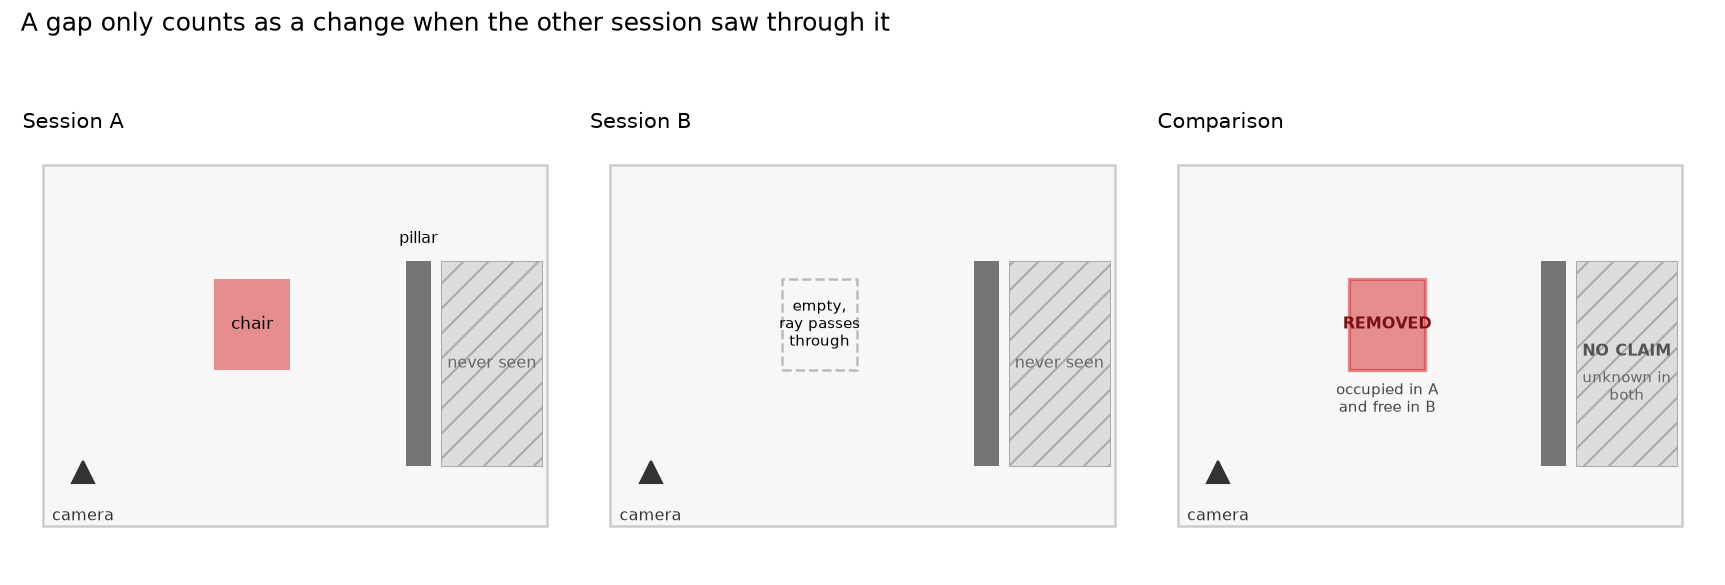
\includegraphics[width=\textwidth]{occupancy_states.png}
\caption{Why the third state matters. The chair is reported as removed because visit B positively
saw through that space. The region behind the pillar is not reported at all, because neither visit
could see it. A system that only tracked occupied space would report both as changes.}
\end{figure}

\begin{plainbox}
That one restriction is the difference between a system that reports \emph{what changed} and one
that reports \emph{where the camera went}.
\end{plainbox}

\section{Group, name, and pair up}

The changed cells are grouped into objects. Each group is then traced back into the photographs
that saw it, cropped out, and shown to CLIP for a name.

One subtle detail matters here. A removed object is cropped from a \textbf{visit A} photograph,
because by visit B it is not there any more.

\begin{watch}
Getting that backwards returns a picture of whatever is sitting in that space now, labels it
confidently, and produces output that is wrong while looking entirely reasonable. Those are the
worst kind of bugs, because nothing about the output announces the error.
\end{watch}

Finally, a disappearance in one place and an appearance in another are reported as a single
\textbf{move} only if they agree on name, are a similar size, and are not too far apart. Otherwise
they stay as two separate events, because that is the honest reading of the evidence.

\chapter{The decisions that mattered}

\section{Reconstructing both visits together}

Covered in Section~4.2. The single most important choice in the project, and the one worth being
able to defend in detail.

\section{Tracking empty space, not just full space}

The thing that stops occlusion being reported as change. Without it the system would be a
difference detector rather than a change detector, and on real footage the difference between
those two is most of the room.

\section{Refusing to answer when the evidence is missing}

The system will miss real changes in parts of the room that only one visit covered. That is
intended, not an oversight.

For a robot, a missed change is a wasted detour. A hallucinated clear path is a collision. Given a
choice between the two failure modes, this one is correct.

\section{Refusing to name things it cannot see properly}

An early version of the report confidently announced that a television had moved. It had not.
There was no television. CLIP was guessing, at a confidence barely distinguishable from random
chance, and the program was printing those guesses as fact.

\begin{plainbox}
With twenty nine candidate labels, a model with no idea scores about $1/29 = 0.034$ for its best
guess. The actual scores coming back were $0.035$. The model was not choosing, it was shrugging.
\end{plainbox}

There is now a floor. Anything scoring near chance is reported as ``unidentified object'', and
moves are not paired on a name nobody believes. The output went from six invented findings to ten
honest ones.

\begin{watch}
This is worth noticing as a general lesson. The system was not broken. It was producing output
that looked exactly like a working system, and only checking the confidence numbers revealed that
the labels were noise.
\end{watch}

\section{Testing against a known answer}

Rather than filming a room and eyeballing the output, the project includes a program that draws a
fake room where the changes are scripted in advance. That makes the results checkable rather than
merely plausible.

\begin{figure}[h]
\centering
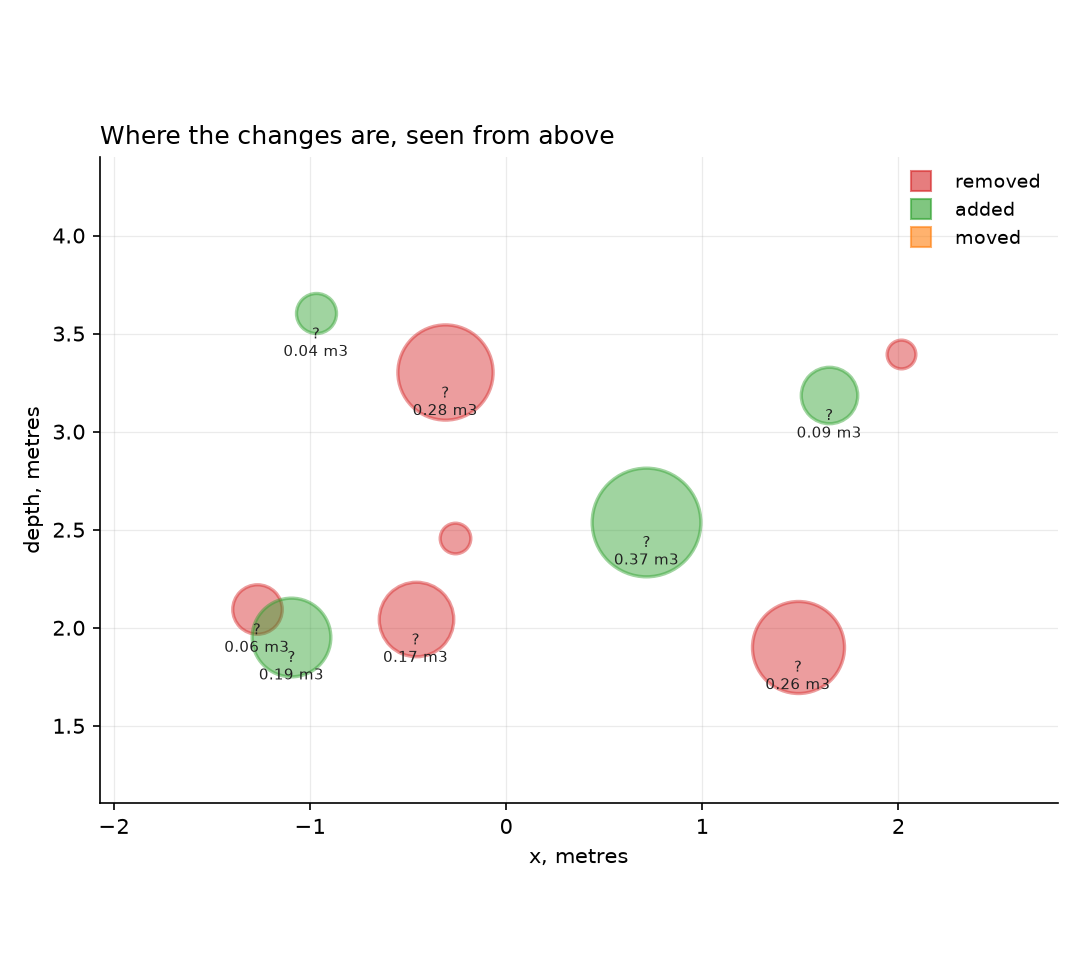
\includegraphics[width=0.92\textwidth]{topdown.png}
\caption{The detected changes seen from above, circle size proportional to volume. The four real
changes land in four different parts of the room, which is what a result tracking real geometry
looks like. A result driven by camera motion would pile up in one corner.}
\end{figure}

\begin{figure}[h]
\centering
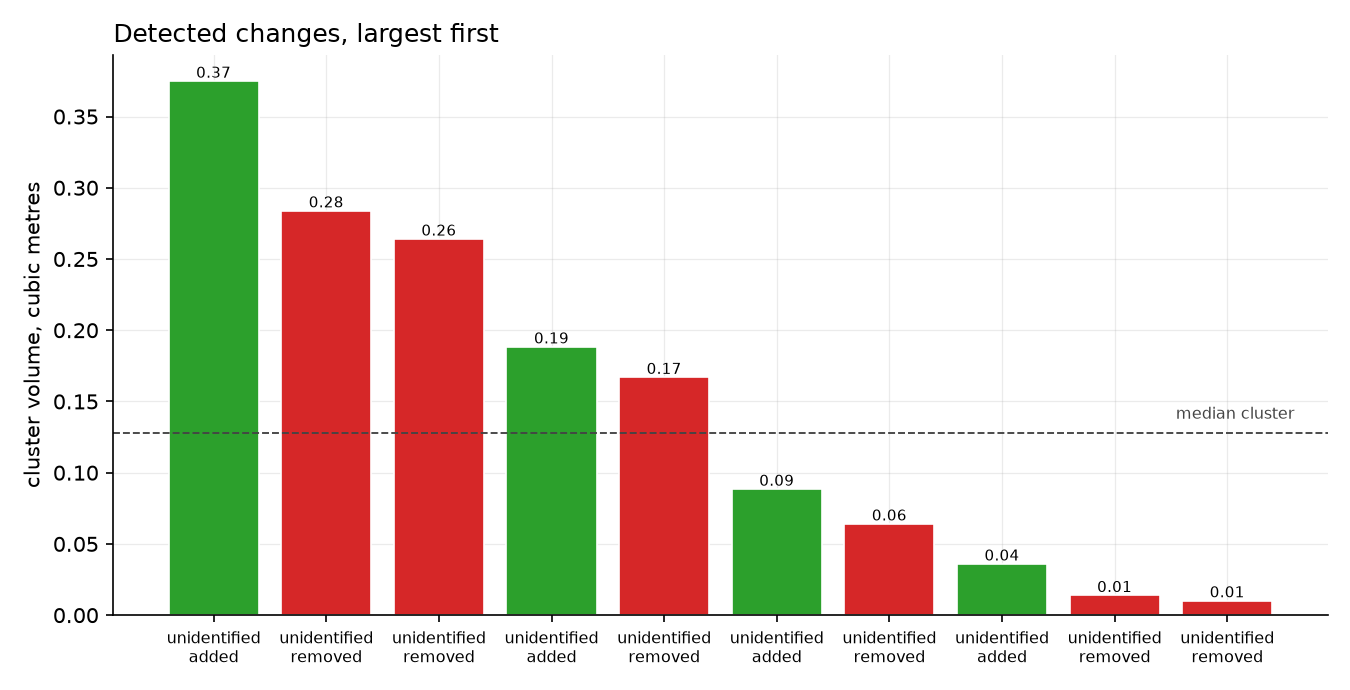
\includegraphics[width=\textwidth]{change_summary.png}
\caption{Every detected cluster by volume. The four real changes are the four largest. Everything
below the median line is depth error on flat walls rather than an object, and it is why a minimum
cluster size exists in the configuration.}
\end{figure}

\chapter{The test room}

\texttt{tools/make\_synthetic\_room.py} draws two videos of an imaginary room from a moving
viewpoint. Between the two, one box moves across the room, one is taken away, one is added, and one
stays exactly where it was.

Because the answer is known in advance, the output can be marked rather than admired.

\section{What the test found}

\begin{center}
\begin{tabular}{@{}p{0.30\textwidth}p{0.22\textwidth}p{0.40\textwidth}@{}}
\toprule
\textbf{Truth} & \textbf{Found} & \textbf{Evidence} \\
\midrule
chair moved left to right & yes & 0.28 m\textsuperscript{3} removed, 0.09 m\textsuperscript{3} added \\[4pt]
box removed from the right & yes & 0.26 m\textsuperscript{3} removed, front right \\[4pt]
bag added on the left & yes & 0.19 m\textsuperscript{3} added, front left \\[4pt]
table unchanged & yes, correctly silent & not reported \\
\bottomrule
\end{tabular}
\end{center}

The volumes are sensible rather than arbitrary. A hollow cube of roughly 0.8 m\textsuperscript{3}
has about 5 m\textsuperscript{2} of surface, and at a five centimetre cell size that is about
0.25 m\textsuperscript{3} of occupied cells, which is what came back.

Six smaller false positives also appear, the largest 0.37 m\textsuperscript{3}. They come from
depth error on large flat walls, where the depth model has little to anchor on. They are the honest
cost of using monocular depth rather than a depth sensor, and they are listed in the project's
README rather than hidden.

\section{Why the test room looks so strange}

The room is covered in colourful noise rather than looking realistic, and that is deliberate.

Reconstruction works by recognising the same distinctive patch of texture in several frames. A
smooth, evenly coloured surface gives it nothing to grip on. A realistic looking render would
reconstruct badly for reasons that have nothing to do with the system being tested, and the test
would be measuring the renderer rather than the pipeline.

\begin{watch}
The honest limitation is that CLIP cannot name a cube covered in coloured noise, so every label on
the synthetic run comes back as ``unidentified object''.

The fake room tests the geometry. Only a real room can test the naming. Saying so plainly is
better than quietly presenting synthetic labels as though they meant something.
\end{watch}

\chapter{Glossary}

\begin{center}
\begin{tabular}{@{}p{0.30\textwidth}p{0.60\textwidth}@{}}
\toprule
\textbf{Term} & \textbf{What it means} \\
\midrule
Structure from motion & Working out three dimensional shape, and where the camera was, from a set of ordinary 2D photographs \\[4pt]
Point cloud & A 3D shape stored as a lot of individual points floating in space \\[4pt]
Sparse and dense & Sparse means a few hundred accurate points per frame. Dense means a depth value for every pixel \\[4pt]
Voxel & A cube shaped cell of 3D space, the three dimensional equivalent of a pixel. Five centimetres across here \\[4pt]
Occupancy map & A record of which cells of space contain something, are known to be empty, or were never seen \\[4pt]
Ray casting & Tracing the straight line from the camera out through a pixel, to find what the camera looked through on the way \\[4pt]
Occlusion & One object hiding another from the camera \\[4pt]
Monocular depth & Estimating distance from a single image, rather than from two views \\[4pt]
Affine-invariant depth & Depth that is correct in relative terms but has unknown scale and offset. It knows nearer and further, not how far \\[4pt]
Zero-shot classification & Naming something using a model that was never specifically trained on that list of names \\[4pt]
Clustering & Grouping scattered measurements into objects \\[4pt]
SIFT keypoint & A distinctive small patch of an image that can be recognised again from a different angle or distance \\[4pt]
Pose & Where the camera was and which way it was pointing \\[4pt]
Least squares & A standard way of finding the line that best fits a set of measurements \\[4pt]
Softmax & Turning a set of raw scores into numbers that behave like probabilities and add up to one \\
\bottomrule
\end{tabular}
\end{center}

\chapter{Questions worth being ready for}

\section{Why not just compare the two point clouds?}

Because absence in a point cloud is ambiguous. It can mean the object left, or it can mean the
camera never looked there. On real footage, where nobody walks the identical route twice, the
second case accounts for most of the room. Tracking confirmed empty space separates the two.

\section{Why one reconstruction instead of aligning two?}

Aligning two models means solving for the transform that makes them agree, and that is least
reliable exactly when part of the scene has moved, which is the only case this project cares
about. Doing it jointly lets the unchanged scene do the aligning, which is the right way round.

\section{How do you know it works?}

A synthetic room with changes scripted in advance. All four are found, in the right places, at
volumes consistent with the surface area of the objects. The figures in Chapter~5 are generated
from that run by code reading the output file, not drawn by hand.

\section{What are the weaknesses?}

Four, stated plainly.

\begin{itemize}
  \item Monocular depth is the weakest link, and its errors are smooth and plausible, which is the
        worst kind of error because nothing looks obviously wrong.
  \item There is no true metric scale, so volumes and distances are consistent but not in real
        metres.
  \item Six false positives appear on the test scene, from depth error on flat walls.
  \item The labelling has only been exercised on noise textured cubes, so it is untested on real
        objects.
\end{itemize}

\section{What would you do next?}

Real metric scale, from a known size marker in shot or from the phone's own motion tracking.
Dense stereo where a GPU is available. Log-odds occupancy, as used in OctoMap, so confidence
accumulates across frames instead of a hard threshold on how many times a cell was hit. An
open-vocabulary detector so objects outside the configured list can still be named.

\section{What did you get wrong along the way?}

Three things, all caught by testing rather than by reading the code.

\begin{enumerate}
  \item \textbf{The depth limit was written in metres while the reconstruction used arbitrary
        units.} The scene reconstructed at roughly twenty eight units deep, the limit was eight, so
        every single measurement was discarded as too far away and nothing fused at all. Fixed by
        rescaling the reconstruction once to room sized units.
  \item \textbf{The first synthetic room had no walls.} Any surface with a single corner behind the
        camera was being discarded whole, which removed the floor and every wall and left a black
        void. Fixed by cutting the large surfaces into tiles so the test applies locally.
  \item \textbf{The naming stage reported guesses as fact,} announcing that a television had moved
        when the model was scoring at chance level. Fixed with a confidence floor.
\end{enumerate}

\begin{plainbox}
All three were invisible from reading the code and obvious from running it against a known answer.
That is the argument for building the synthetic test room before trusting anything.
\end{plainbox}


\end{document}
